\chapter*{Niveau 1}
\addcontentsline{toc}{chapter}{Niveau 1}
Du har lært at brygge lette drikke. Mange urter viser tydeligt deres potentiale, og du kan hjælpe dine venner i kamp.
\begin{table}[H]
    \centering
    \begin{tabular}{|p{0.50\textwidth}|p{0.25\textwidth}|}
    \rowcolor{cerulean!80}\hline
        Evne navn & Pris i XP \\\hline
         Alkymi Niv. 1 & 1 \\\hline
         Indkomst & 1 \\\hline
         Kemisk våben & 2 \\\hline
         Læse/Skrive Elvisk & 1\\
         \hline
    \end{tabular}
\end{table}

\section*{Evne beskrivelse}
\addcontentsline{toc}{section}{Evne beskrivelse}

\subsection*{Alkymi Niv. 1}
\addcontentsline{toc}{subsection}{Alkymi Niv. 1}
Du kan nu brygge en af de nedenstående drikke. Alle disse drikke kræver specifikke ingredienser, og kun du kan blande dem korrekt.\\

\begin{table}[H]
    \centering
    \begin{tabular}{|c|c|}
        \rowcolor{cerulean!80}\hline
        Drik & Gift \\\hline
        Enkens tåre &  Dværge snaps \\\hline
        Naturens bryg & Nervegift \\\hline
        Sten næver &  \\\hline
    \end{tabular}
    \caption{Oversigt over niveau 1 drikke.}
\end{table}

\begin{gift*}[Dværge snaps]
\textbf{Type:} Negativ Gift\\
\textbf{Ingredienser:} Øl fra kroen \& Vorterod\\
\textbf{Indtagelse:} Drikkes\\
\textbf{Effekt:} Ved indtagelse bliver man øjeblikkeligt meget beruset. Virkningen forsvinder, hvis spilleren mister bevidstheden eller 15 min efter indtagelse. Drikke efterlader ingen tømmermænd.\\
\end{gift*}

\begin{drik*}[Enkens tåre]
\textbf{Type:} Øjeblikkelig Drik\\
\textbf{Ingredienser:} Kongetand \& rent vand\\
\textbf{Indtagelse:} Drikkes\\
\textbf{Effekt:} Denne drik fjerne alle effekter af alkohol og gør øjeblikkeligt spilleren ædru. Dette betyder at de ikke vil være påvirket af alkohollet eller evner der kræver man er under effekten for alkohol.\\
\end{drik*}

\begin{drik*}[Naturens bryg]
    \textbf{Type:} Øjeblikkelig Drik\\
    \textbf{Ingredienser:} Ingen\\
    \textbf{Indtagelse:} Drikkes\\
    \textbf{Effekt:} Denne drik helbreder 1 LP. Du kan aldrig blive helbredt for mere end dit max LP.\\
    \textbf{Særligt:} Denne drik kan brygges hver anden time, men vare kun til slutningen af scenariet.
\end{drik*}

\begin{gift*}[Nervegift]
    \textbf{Type:} Øjeblikkelig Gift\\
    \textbf{Ingredienser:} Ingen\\
    \textbf{Indtagelse:} Drikkes / Blandes med væske\\
    \textbf{Effekt:}Denne drik skader 1 LP, og kan blandes i andre drikke uden, at den mister sin virkning.\\
   \textbf{Særligt:} Denne drik kan brygges hver anden time, men vare kun til slutningen af scenariet.
\end{gift*}

\begin{drik*}[Sten næver]
\textbf{Type:} Positiv drik\\
\textbf{Ingredienser:} 1 Dværgerod.\\
\textbf{Indtagelse:} Drikkes\\
\textbf{Effekt:} Når du drikker denne drik, får du +2NK i 30 min.
\end{drik*}


\subsection*{Indkomst}
\addcontentsline{toc}{subsection}{Indkomst}
Rul en 6-sidet terning ved tjek-in og få den mængde i Fjend\footnote{Møntfoden i A'kastin.} udleveret.

\subsection*{Kemisk våben}
\addcontentsline{toc}{subsection}{Kemisk våben}
Du kan nu påføre en gift på dit eget Våben. Det skal være et våben med klinge dvs. kniv, sværd eller lignende. Når du slår en person med dette våben vil ofret blive ramt af alle effekter som din gift har. Du kan kun ramme ét offer med giften, før en ny skal påføres. Du kan ikke give dit gift våben til andre. Vær opmærksom på at hvis du har den generelle evne, 'Påfør gift' vil du få XP prisen tilbage fra den evne når du køber Kemisk våben.\\

\subsection*{Læse/Skrive Elvisk}
\addcontentsline{toc}{subsection}{Læse/Skrive Elvisk}
Du kan læse og skrive skrift, der er skrevet på Elvisk.\\
\begin{figure}[H]
    \centering
    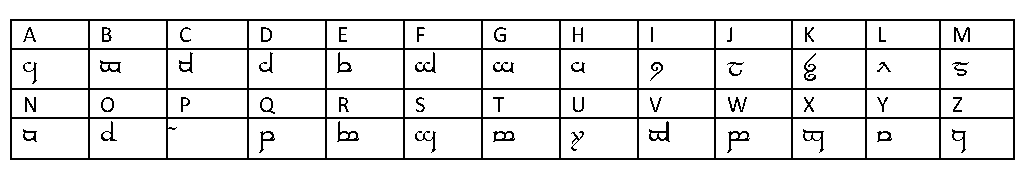
\includegraphics[width=1\textwidth]{setup/Alfabeter/Elvisk alfabet.pdf}
    \caption{Elvisk alfabet}
\end{figure}

